% !TeX spellcheck = it_IT
\documentclass{beamer}
\usepackage[italian]{babel}
\usepackage[normalem]{ulem}
\usepackage{tikz}
\usetikzlibrary{shapes.geometric, arrows, arrows.meta, automata, positioning, quotes}
\tikzstyle{box} = [rectangle, minimum width=5cm, minimum height=1cm, text centered,text width=5cm, draw=black, fill=white!30]
\tikzstyle{box2} = [rectangle, minimum width=2cm, minimum height=3cm, text centered,text width=2cm, draw=black, fill=white!30]
\tikzstyle{box3} = [rectangle, minimum width=3cm, minimum height=1cm, text centered,text width=3cm, draw=black, fill=white!30]
\tikzstyle{decision} = [diamond, minimum width=1cm, minimum height=1cm, text centered, text width=2cm, draw=black, fill=white!30]
\tikzstyle{arrow} = [thick,->,>=stealth]
\usepackage{chronosys}
\usetheme{Madrid}
\setbeamertemplate{navigation symbols}{}
\title[La storia del DRM]{La storia del DRM}
\subtitle{Un viaggio nel passato delle tecnologie anti-pirateria}
\author[scudo, neonsn0w]{Leonardo 'scudo' Rossi \newline Pietro 'neonsn0w' Prase}
\date[ESC\{21\}]{End Summer Camp 21, 6 settembre 2025}
\begin{document}
	\frame{\titlepage}
	\begin{frame}
		\frametitle{Introduzione}
		\textbf{Digital Rights Management:}\newline
		\begin{itemize}
			\item Set di tecnologie hardware e software
			\item Impedire o rilevare copia non autorizzata di informazioni (software, musica, film...)
			\item Tratteremo solo il software
		\end{itemize}
	\end{frame}
	\begin{frame}
		\frametitle{Timeline}
		\fontsize{6}{8} Periodi di dominanza dei vari canali di distribuzione del software:\newline\newline\newline
		\startchronology[startyear=1975,color=blue,width=0.9\textwidth,height=5ex,dates=false]
		\tiny
		\chronoperiode[textdepth=-30px]{1975}{1993}{\textbf{Cartucce, cassette e floppy}}
		\chronoevent[markdepth=20px,barre=false]{1988}{CD-ROM}
		\chronoperiode[textdepth=-30px,startdate=false]{1993}{2013}{\textbf{Dischi ottici}}
		\chronoevent[markdepth=20px,barre=false]{1997}{DVD-ROM}
		\chronoevent[markdepth=20px,barre=false]{2003}{Steam}
		\chronoperiode[textdepth=-30px,stopdate=false]{2013}{2025}{\quad\quad \textbf{Distribuzione digitale}}
		\stopchronology
	\end{frame}
	\begin{frame}
		\frametitle{Cartucce}
		\textbf{Caratteristiche:}\newline
		\begin{itemize}
			\item Comuni fra le console (ma presenti su alcuni computer)
			\item Memoria ROM o flash
			\item Possibilità di aggiungere hardware specializzato (es. CIC)
			\item Iniziale importanza di fermare software non approvato
		\end{itemize}
	\end{frame}
	\begin{frame}
		\frametitle{Cartucce}
		\begin{figure}[h]
			\centering
			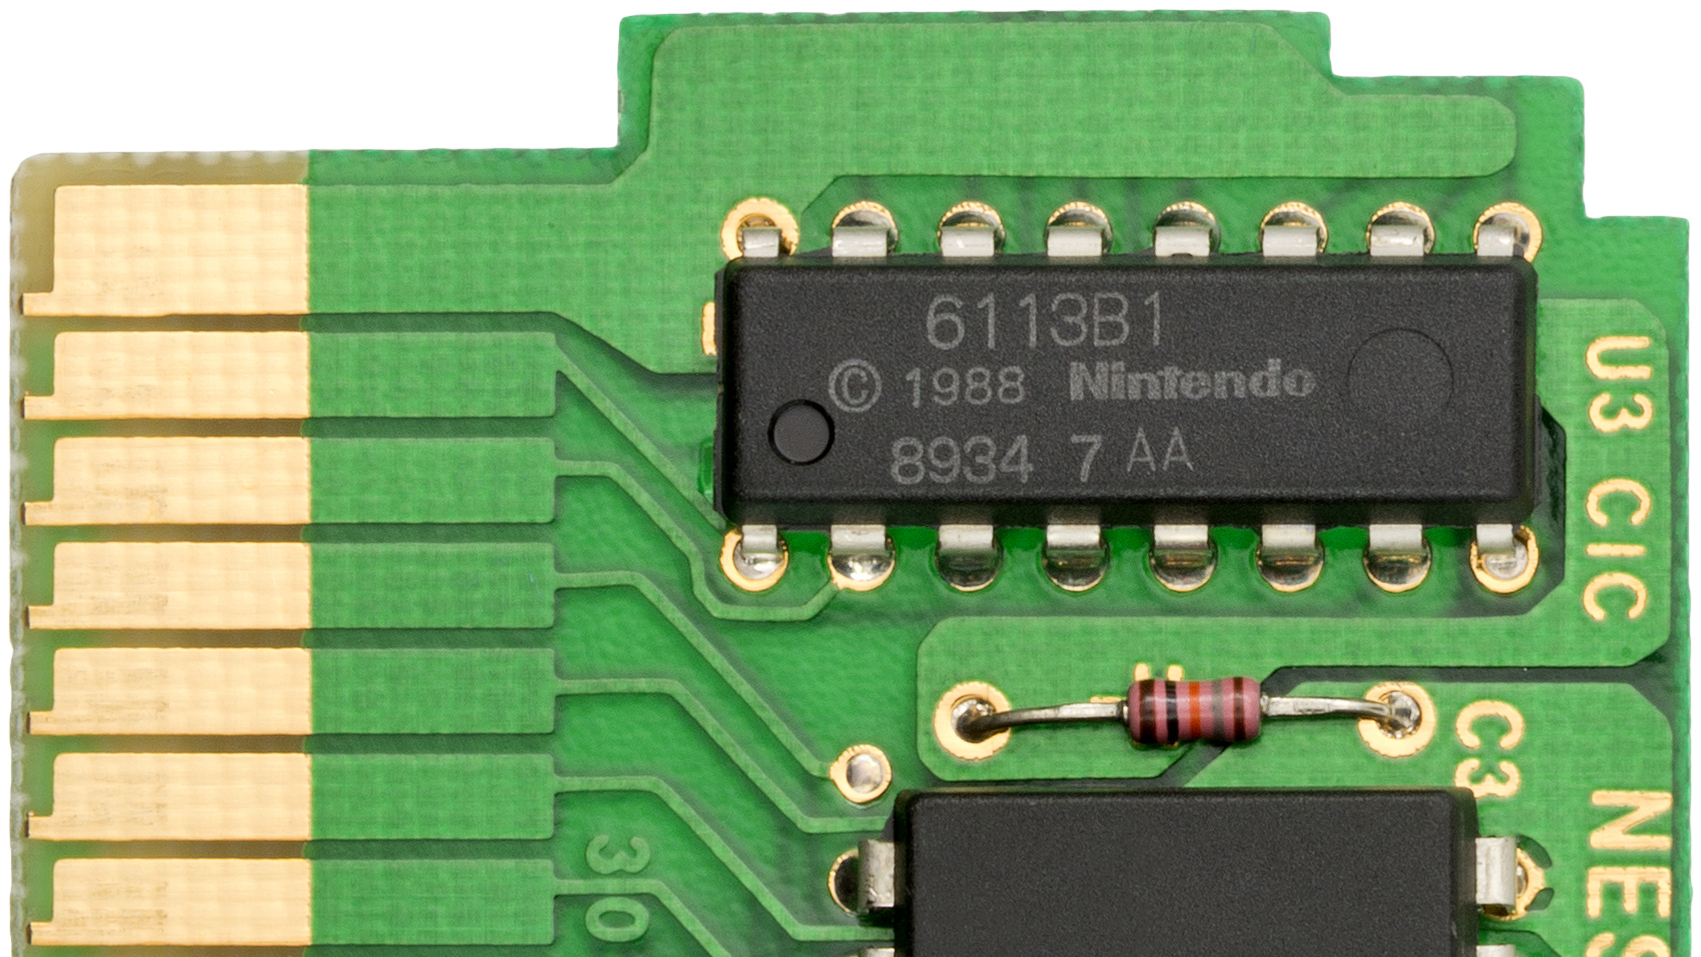
\includegraphics[width=0.85\textwidth]{imgs/cic.jpg}
			\caption{Un chip CIC usato nel Nintendo Entertainment System.}
			\label{pic:nes_cic}
		\end{figure}
	\end{frame}
	\begin{frame}
		\frametitle{Cartucce}
		\textbf{Problemi delle cartucce:}\newline
		\begin{center}
			\begin{tikzpicture}[node distance=2cm]
				\node (att) [box, thick] {DRM hardware bypassabile con attacchi specializzati};
				\node (fl) [box, below of=att,thick] {Flashcard (R4, Sky3DS, MIG-Switch)};
				\draw [arrow, ultra thick] (att) -- (fl);
			\end{tikzpicture}
		\end{center}
		\begin{itemize}
			\item Meglio usare tecniche crittografiche (firmare e criptare il software)
			\item Formato generalmente in disuso (alti costi di produzione)
		\end{itemize}
	\end{frame}
	\begin{frame}
		\frametitle{Floppy disk}
		\textbf{Caratteristiche:}\newline
		\begin{itemize}
			\item Comuni nei computer (ma presenti su alcune console)
			\item Disco magnetizzato rotante
			\item Inizialmente più formati, che convergono $\to$ rampante pirateria
		\end{itemize}
	\end{frame}
	\begin{frame}
		\frametitle{Floppy disk}
		È possibile identificare alcune tecniche comuni:\\[20pt]
		\begin{itemize}
			\item Settori allocati in modo non standard (rimappati)
			\item Disco formattato in modo non standard (custom fs: più dati)
			\item Uso di \textit{fuzzy bits} (informazioni magnetiche con stato non definito)\\[20pt]
		\end{itemize}
		In genere si cercano caratteristiche che può avere solo un floppy originale.
	\end{frame}
	\begin{frame}
		\frametitle{Altri tipi di protezione}
		Altre tecniche meno comuni cadute in disuso sono:\newline
		\begin{itemize}
			\item \textit{Codewheel} 
			\item Protezioni basate sul manuale (ricerca di parole)
			\item \textit{Dongle} di vario tipo\\[20pt]
		\end{itemize}
		Quindi oggetti fisici venduti assieme al gioco.
	\end{frame}
	\begin{frame}
		\frametitle{Altri tipi di protezione}
		\begin{figure}[h]
			\centering
			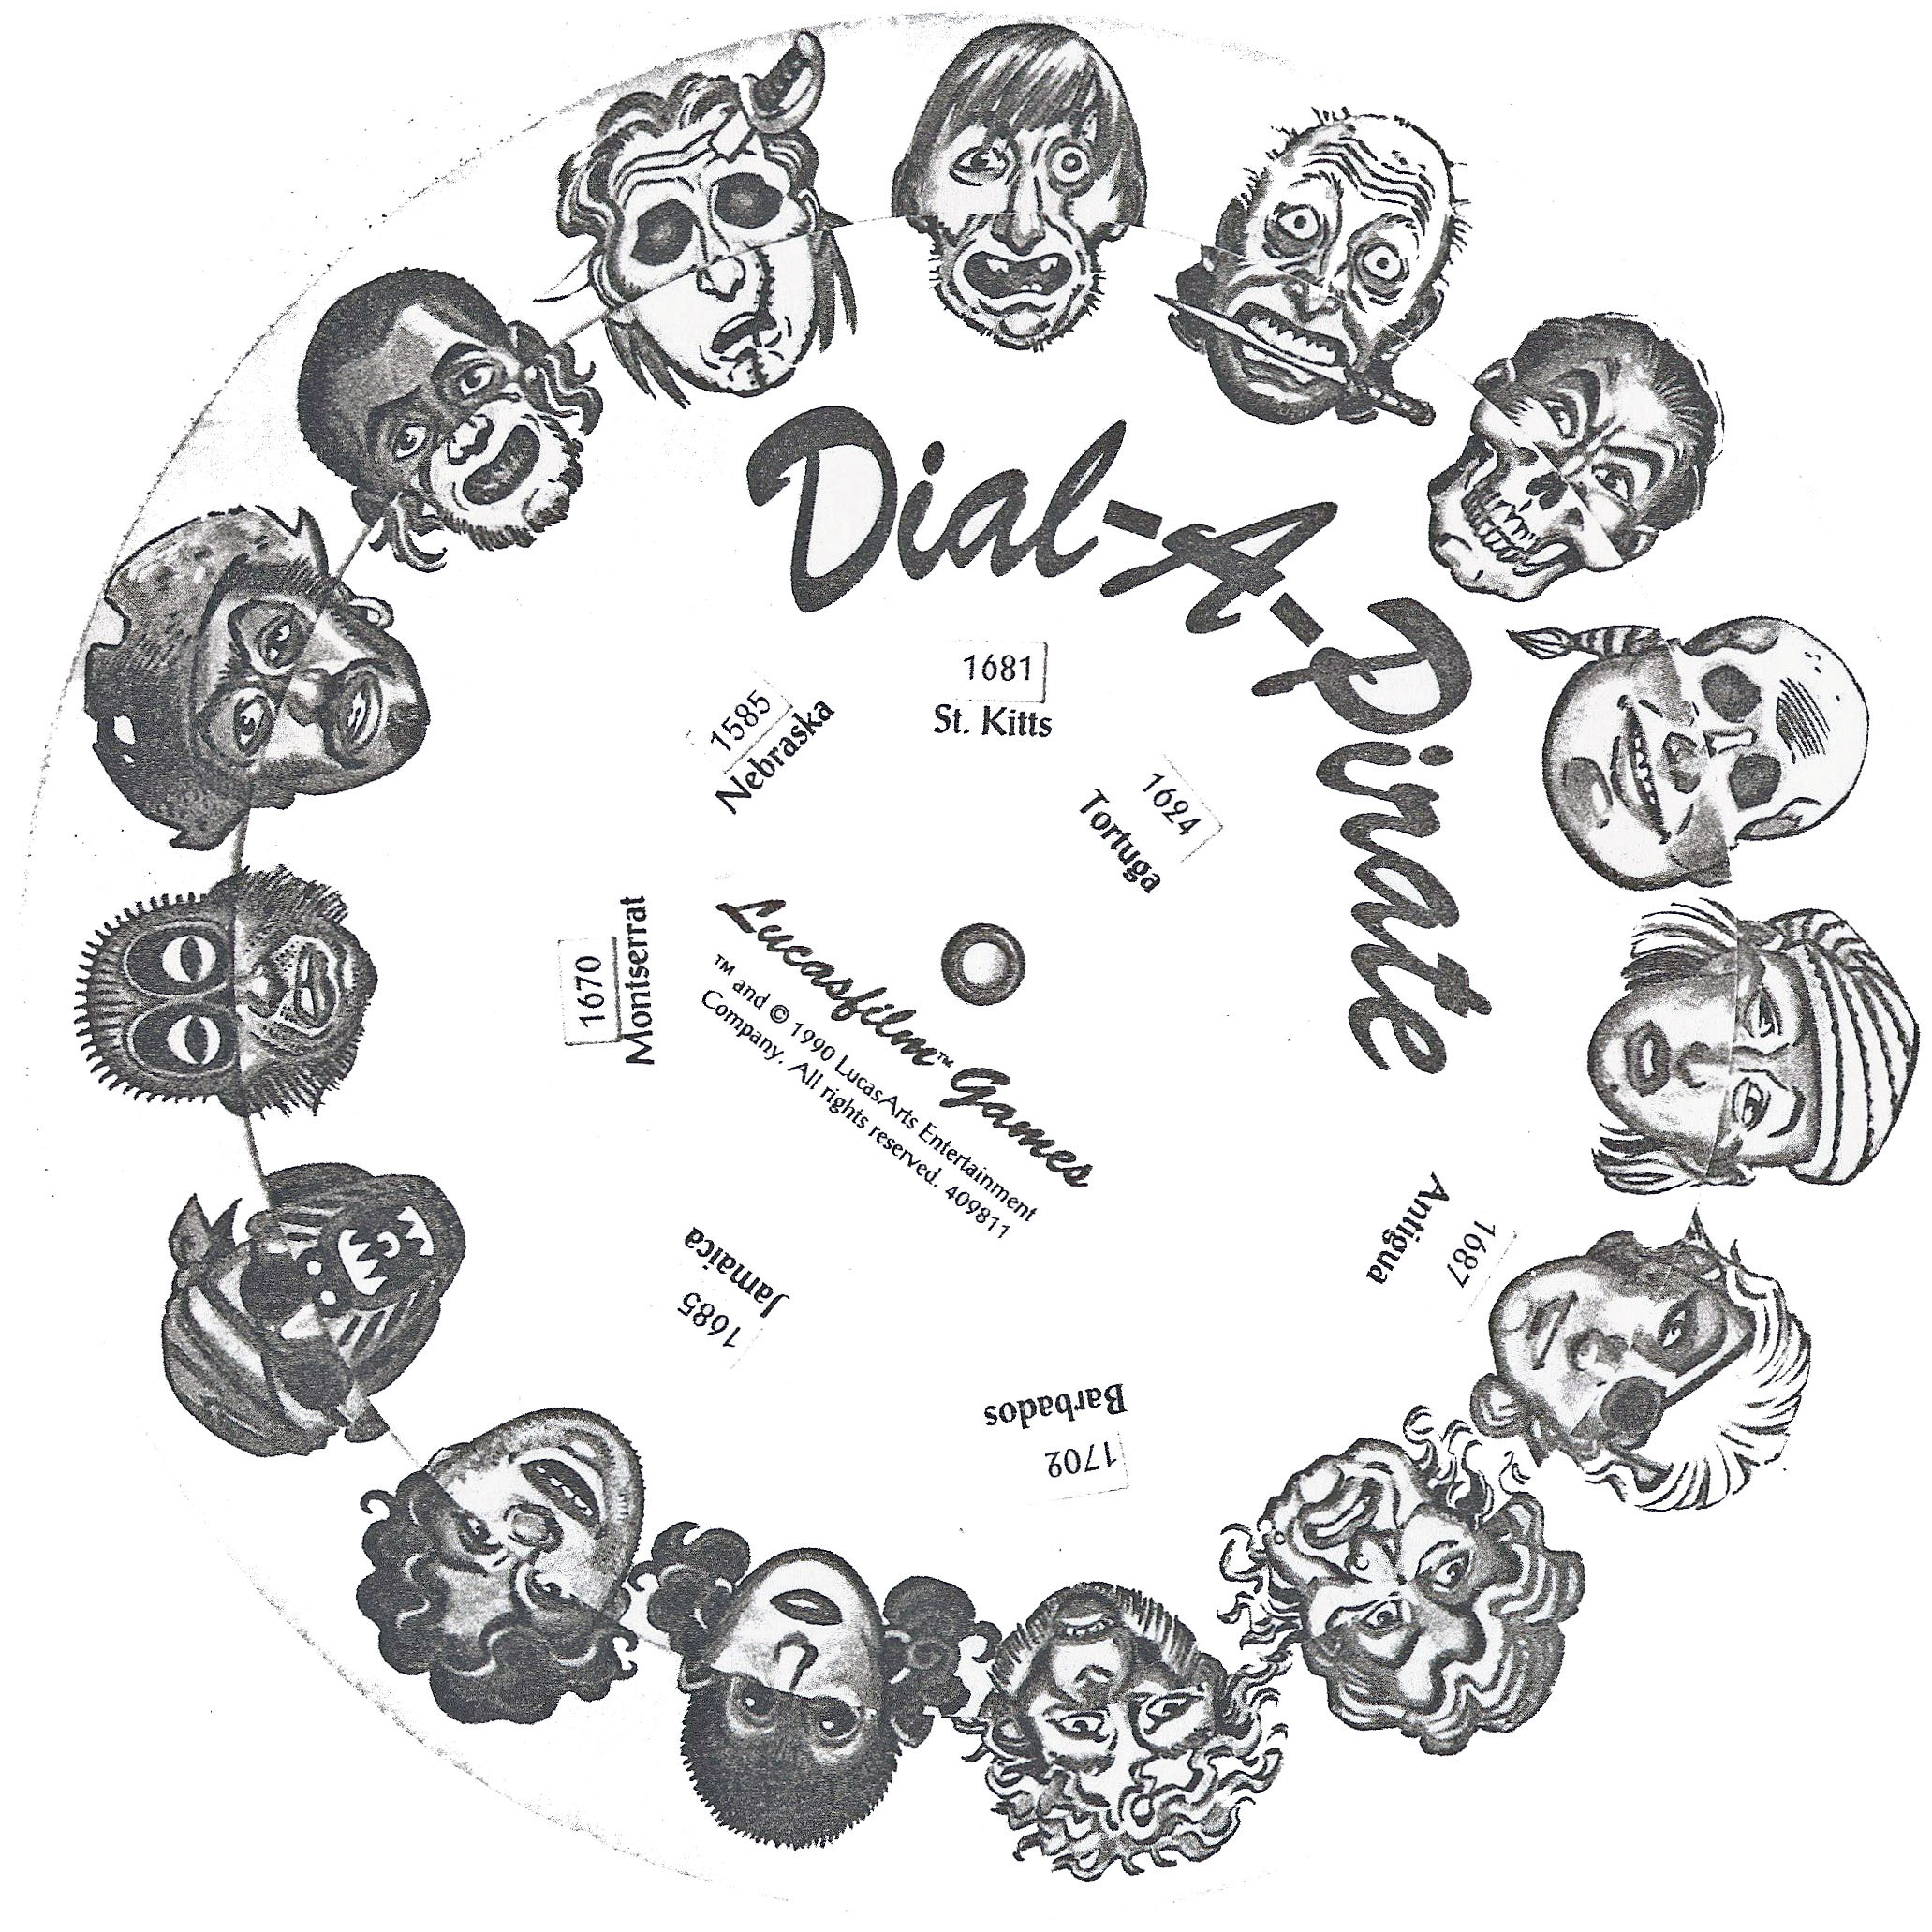
\includegraphics[width=0.5\textwidth]{imgs/codewheel.jpg}
			\caption{Un \textit{codewheel}.}
			\label{pic:codewheel}
		\end{figure}
		\begin{center}
			\scriptsize Questa foto di Paul Downey è rilasciata sotto licenza CC BY 2.0.
		\end{center}
	\end{frame}
	\begin{frame}
		\frametitle{Optical media good}
		Nei primi anni del CD-ROM, \textbf{non si pose il problema della copia pirata}.
		\begin{itemize}
			\item I masterizzatori erano ancora molto costosi ($>$20.000\$!)
			\item Tecniche anti-copia rudimentali:
			\begin{itemize}
				\item Fake TOC (Table of Contents)
				\item CD-ROM più capienti del normale
			\end{itemize}
		\end{itemize}
	\end{frame}
	\begin{frame}
		\frametitle{CD-ROM più capienti}
		CD "pressati" con capacità più ampia di un CD-R $\to$ impedire la copia.\\
		Approccio fallato:
		\begin{itemize}
			\item Spesso c'era molto "filler" rimovibile
			\item \textbf{Overburning} 
		\end{itemize}
		\begin{figure}
			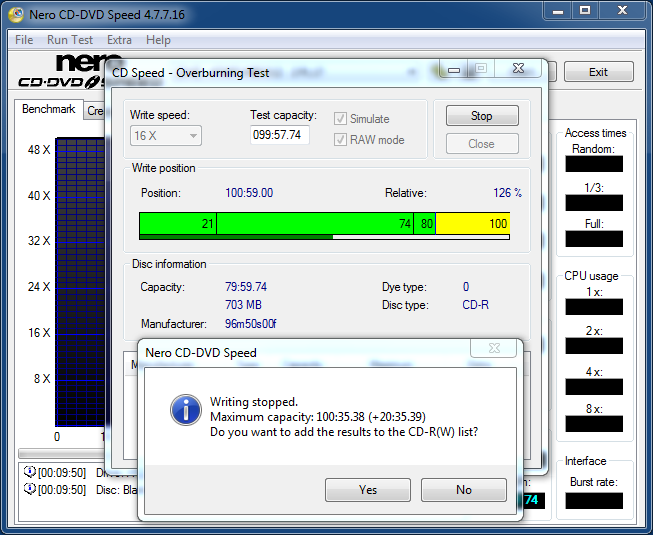
\includegraphics[width=0.45\textwidth]{imgs/nero.png}
		\end{figure}
	\end{frame}
	\begin{frame}
		\frametitle{SecuROM}
		\textbf{SecuROM} era uno dei primi DRM sofisticati per CD
		\begin{itemize}
			\item Creato da \textbf{Sony}
			\item \textbf{Chiave univoca} per ogni CD, non copiabile da un drive
			\item \textbf{Parti dell'eseguibile criptate}, decriptate all'esecuzione con la chiave univoca e un driver kernel
			\item \textbf{Il disco doveva essere nel PC per eseguire il software}
		\end{itemize}
		\,\newline
		\begin{figure}
			
\includegraphics[width=0.55\textwidth]{imgs/SecuROM_logo.png}
		\end{figure}
	\end{frame}
	\begin{frame}
		\frametitle{SecuNOT}
		SecuROM fallì nel suo intento:
		\begin{itemize}
			\item Era possibile \textbf{leggere l'eseguibile decriptato} con un debugger
			\item Nacquero le crack "\textit{NoCD}"
		\end{itemize}
		\, \newline
		In compenso, \textbf{anche chi possedeva la copia originale del disco riscontrava problemi...}
		\begin{itemize}
			\item A volte il disco non veniva rilevato
			\item Problemi su Windows Vista
			\item SecuROM \textbf{non funzionava} con certi drive
		\end{itemize}
	\end{frame}
	\begin{frame}
		\frametitle{SecuROM + Attivazione Online}
		\begin{columns}
			\begin{column}{0.6\textwidth}
				Con l'uscita di Spore, EA aggiunse a SecuROM un sistema di \textbf{attivazione online}.
				Questo approccio era \textbf{un inferno}:
				\begin{itemize}
					\item Connessione a internet obbligatoria
					\item Numero di attivazioni limitato
					\item Ogni modifica hardware rendeva necessaria un'ulteriore attivazione
				\end{itemize}
				EA fu costretta a rimuovere SecuROM da Spore in seguito ad un'azione legale
			\end{column}
			\begin{column}{0.4\textwidth}
				\begin{figure}[h]
					\centering
					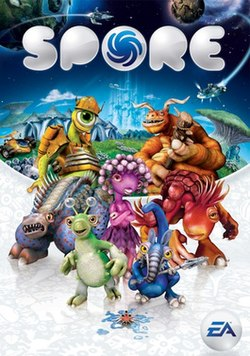
\includegraphics[width=0.8\textwidth]{imgs/Sporebox.jpg}
					\caption{Spore (2008)}
				\end{figure}
			\end{column}
		\end{columns}	
	\end{frame}
	\begin{frame}
		\frametitle{StarForce}
		DRM \textbf{molto sofisticato}.
		\begin{itemize}
			\item Sviluppato da \textbf{Protection Technology}
			\item Approccio multi-tier
			\item Moltissimi file nel disco erano criptati
			\item Ogni disco aveva dei parametri univoci
		\end{itemize}
		\begin{figure}
			
\includegraphics[width=0.45\textwidth]{imgs/Starforce_logo.png}
		\end{figure}
		Assomiglia a SecuROM, ma ci sono delle differenze fondamentali
	\end{frame}
	\begin{frame}
		\frametitle{StarForce}
		StarForce installa driver \textbf{Ring 0 (kernel)}, che gestiscono il drive.
		\begin{figure}
			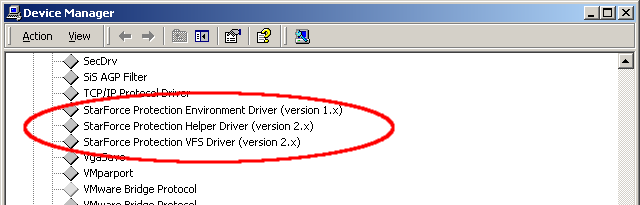
\includegraphics[width=0.8\textwidth]{imgs/Starforce_drivers.png}
		\end{figure}
		Il driver VFS gestisce il \textit{virtual filesystem}
	\end{frame}
	\begin{frame}
		\frametitle{StarForce VFS}
		Il VFS è composto da:
		\begin{itemize}
			\item dei file "container" che contengono i dati di gioco
			\item il driver usato per accedere ai dati di gioco (sfvfs02.sys)
		\end{itemize}
		\begin{center}
			\begin{tikzpicture}[node distance=3cm]
				\node (serv) [box2, thick] {Eseguibile};
				\node (client) [box2, right of=serv,thick, xshift=3cm] {VFS con file di gioco criptati};
				\draw[arrow, <->] (serv) -- node[fill=white]{sfvfs02.sys} (client);
			\end{tikzpicture}
		\end{center}
		Il VFS viene quindi usato per nascondere i file di gioco.
	\end{frame}
	\begin{frame}
		\frametitle{StarForce}
		\begin{columns}
			\begin{column}{0.6\textwidth}
				StarForce fu molto efficace. \newline \newline
				\textit{Splinter Cell: Chaos Theory} fu craccato solo dopo \textbf{422 giorni}.
				\newline \newline
				Tuttavia, i problemi non mancavano...
			\end{column}
			\begin{column}{0.4\textwidth}
				\begin{figure}[h]
					\centering
					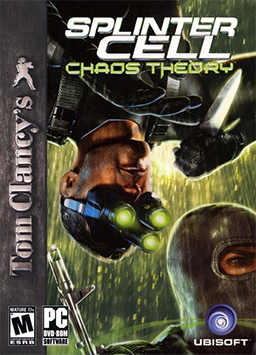
\includegraphics[width=0.8\textwidth]{imgs/SCCT_Coverart.png}
				\end{figure}
			\end{column}
		\end{columns}	
	\end{frame}
	\begin{frame}
		\frametitle{Uh oh...}
		\begin{itemize}
			\item Incompatibilità con Vista e successivi
			\item Instabilità anche su XP
			\item StarForce non era menzionato nell'EULA
			\item Driver Ring 0 installati senza avvisare l'utente
			\begin{itemize}
				\item Rimanevano dopo la rimozione del gioco
				\item StarForce Removal Tool non sempre funzionava
			\end{itemize}
			\item Non era possibile avere più di un drive
			\item DMA disabilitato
			\item Problemi con dischi non StarForce
			\item \textbf{Danneggiamento del drive}
		\end{itemize}
	\end{frame}
	\begin{frame}
		\frametitle{Windows 10}
		\begin{columns}
			\begin{column}{0.6\textwidth}
				Nel 2015, con l'uscita di Windows 10, Microsoft annunciò che i vecchi giochi che usavano dei DRM che agivano sul kernel (SecuROM, StarForce, SafeDisc, ecc.) non avrebbero più funzionato per motivi di sicurezza.
			\end{column}
			\begin{column}{0.4\textwidth}
				\begin{figure}[h]
					\centering
					
\includegraphics[width=1\textwidth]{imgs/win10logo.png}
				\end{figure}
			\end{column}
		\end{columns}	
	\end{frame}
	\begin{frame}
		\frametitle{Distribuzione digitale}
		\textbf{Caratteristiche:}\newline
		\begin{itemize}
			\item Vendita e distribuzione via Internet direttamente al cliente
			\item Rimozione dei costi di produzione (supporto fisico usato come token)
			\item Invio di patch in tempo reale (niente richiami di prodotto)
			\item Inizialmente solo su PC, poi anche su console
			\item Forte spinta dopo il successo di Steam
		\end{itemize}
	\end{frame}
	\begin{frame}
		\frametitle{Distribuzione digitale}
		\textbf{Varie tecnologie:}\newline
		\begin{itemize}
			\item Collegamenti con account online proprietari
			\item Sistemi DRM always-online
			\item Uso di virtualizzazione e offuscamento\newline
		\end{itemize}
	\end{frame}
	\begin{frame}
		\frametitle{Distribuzione digitale - Ticket}
		\textbf{Ticket:} piccoli file che contengono una "autorizzazione" firmata crittograficamente che certifica che chi ne è in possesso puó utilizzare quel software.\newline
		\begin{center}
			\begin{tikzpicture}[node distance=3cm]
				\node (serv) [box2, thick] {Black box sicura};
				\node (client) [box2, right of=serv,thick, xshift=3cm] {Software (vuole sapere se è legit)};
				\draw[arrow] (4.9,0.5) -- node[fill=white]{Invio del ticket} (1.1,0.5);
				\draw[arrow] (1.1,-0.5) -- node[fill=white]{Validità del ticket} (4.9,-0.5);
			\end{tikzpicture}
		\end{center}Es.
		\begin{itemize}
			\item IOS (Wii)
		\end{itemize}
	\end{frame}
	\begin{frame}
		\frametitle{Distribuzione digitale - Account online}
		\begin{center}
			\begin{tikzpicture}[node distance=0.5cm]
				\node (process)[box3]{Software invia richiesta di autorizzazione};
				\node (decision)[decision, below=of process]{L'account "possiede" questo software?};
				\node (out1)[box3, below left of=decision, xshift=4cm, yshift=-2cm]{Non avviare il software};
				\node (out2)[box3, below right of=decision, xshift=-4cm, yshift=-2cm]{Richiedi ticket e avvia software};
				\draw [arrow] (process) -- (decision);
				\draw [arrow] (decision) -| node[fill=white]{N} (out1);
				\draw [arrow] (decision) -| node[fill=white]{Y}(out2);
			\end{tikzpicture}
		\end{center}
	\end{frame}
	\begin{frame}
		\frametitle{Distribuzione digitale - Sistemi \textit{always-online}}
		\textbf{Funzionamento:}\newline
		\begin{itemize}
			\item Controllo account all'avvio
			\item Controllo ticket periodico con il server
			\item Errore di connessione/verifica fallita $\to$ chiusura software
			\item Spesso collegato con anticheat
		\end{itemize}
	\end{frame}
	\begin{frame}
		\frametitle{Distribuzione digitale - Virtualizzazione e offuscamento}
		\textbf{Funzionamento:}\newline
		\begin{itemize}
			\item Sezioni dell'eseguibile criptate e/o offuscate
			\item Decriptazione/deoffuscamento grazie al ticket
			\item Ticket collegato ad autenticazione con server DRM
			\item Uso di VM proprietarie (VMProtect, Denuvo)
		\end{itemize}
	\end{frame}
	\begin{frame}
		\frametitle{Crediti e ringraziamenti}
		\begin{center}
			\huge Domande?
		\end{center}
	\end{frame}
\end{document}